\section{Příklad 3}
% Jako parametr zadejte skupinu (A-H)
\tretiZadani{A}


\begin{figure}[H]
    \centering
    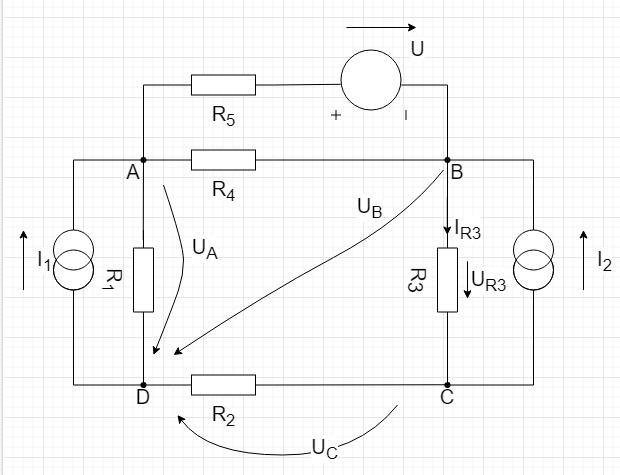
\includegraphics[scale=0.5]{picturesFor3Uloha/1.png}
    \begin{quote}
        \centering
	   $\phi D = 0$ \\~\\
	   $I_1 - I_{R1} - I_{R4} - I_{R5} = 0$ \\
	   $I_{R5} + I_{R4} + I_2 - I_{R3} = 0$ \\
	   $I_{R3} - I_2 - I_{R2} = 0$ \\
    \end{quote}
\end{figure}

\newpage
\begin{quote}
    \centering
    $I_{R1} = \dfrac{(\phi D + \phi A)}{R_1} = \dfrac{\phi A}{R_1} $ \\~\\
    $I_{R2} = \dfrac{(\phi C - \phi D)}{R_2} = \dfrac{\phi C}{R_2} $ \\~\\
    $I_{R3} = \dfrac{(\phi B - \phi C)}{R_3} $ \\~\\
    $I_{R4} = \dfrac{(\phi A - \phi B)}{R_4} $ \\~\\
    $I_{R5} = \dfrac{(\phi A - \phi B - U)}{R_5} $ \\~\\ 
\end{quote}

\begin{quote}
    \medskip
    \medskip
    \centering
    $I_1 - \dfrac{\phi A}{R_1} - \dfrac{\phi A - \phi B}{R_4} - \dfrac{(\phi A - \phi B - U)}{R_5} = 0$ \\~\\ 
    $I_2 + \dfrac{\phi A - \phi B}{R_4} + \dfrac{(\phi A - \phi B - U)}{R_5} - \dfrac{(\phi B - \phi C)}{R_3} = 0$ \\~\\
    $ \dfrac{(\phi B - \phi C)}{R_3} - I_2 - \dfrac{\phi C}{R_2} = 0$ \\~\\
\end{quote}

\begin{quote}
    \medskip
    \medskip
    \centering
    $I_1 - \dfrac{\phi A}{R_1} -  \dfrac{\phi A}{R_4} + \dfrac{\phi B}{R_4} - \dfrac{\phi A}{R_5} + \dfrac{\phi B}{R_5} + \dfrac{U}{R_5}= 0$ \\~\\ 
    $I_2 + \dfrac{\phi A}{R_4} -  \dfrac{\phi B}{R_4} + \dfrac{\phi A}{R_5} - \dfrac{\phi B}{R_5} - \dfrac{U}{R_5} - \dfrac{\phi B}{R_3} + \dfrac{\phi C}{R_3}= 0$ \\~\\ 
    $\dfrac{\phi B}{R_3} - \dfrac{\phi C}{R_3} - I_2 - \dfrac{\phi C}{R_2} = 0$ \\~\\ 
\end{quote}

\begin{quote}
    \medskip
    \medskip
    \centering
    $-\phi A * (\dfrac{1}{R_1} +  \dfrac{ 1}{R_4} + \dfrac{1}{R_5}) + \phi B * (\dfrac{ 1}{R_4} + \dfrac{ 1}{R_5})  = -I_1 - \dfrac{U}{R_5}$ \\~\\ 
    $\phi A * (\dfrac{1}{R_4} + \dfrac{1}{R_5}) - \phi B * (\dfrac{1}{R_4} + \dfrac{1}{R_5} + \dfrac{1}{R_3}) + \phi C * (\dfrac{1}{R_3})  = -I_2 + \dfrac{U}{R_5}$ \\~\\
    $\phi B * (\dfrac{1}{R_3}) - \phi C * (\dfrac{1}{R_3} + \dfrac{1}{R_2})  = I_2 $ \\~\\
\end{quote}


\begin{quote}
    \medskip
    \medskip
    \centering
    $-\phi A * (\dfrac{1}{53\Omega} +  \dfrac{ 1}{39\Omega} + \dfrac{1}{32\Omega}) + \phi B * (\dfrac{ 1}{39\Omega} + \dfrac{ 1}{32\Omega})  = -0.9\Am - \dfrac{120\Vo}{32\Omega}$ \\~\\ 
    $\phi A * (\dfrac{1}{39\Omega} + \dfrac{1}{32\Omega}) - \phi B * (\dfrac{1}{39\Omega} + \dfrac{1}{32\Omega} + \dfrac{1}{65\Omega}) + \phi C * (\dfrac{1}{65\Omega})  = -0.7\Am + \dfrac{120\Vo}{32\Omega}$ \\~\\
    $\phi B * (\dfrac{1}{65\Omega}) - \phi C * (\dfrac{1}{65\Omega} + \dfrac{1}{49\Omega})  = 0.7\Am $ \\~\\
\end{quote}

\begin{quote}
    \medskip
    \medskip
    \centering
    $-\phi A * (0.0757) + \phi B * (0.0568)  = -4.65$ \\~\\ 
    $\phi A * (0.0568) - \phi B * (0.0722) + \phi C * (0.0153)  =3.05$ \\~\\
    $\phi B * (0.0153) - \phi C * (0.0357)  = 0.7    $ \\~\\
\end{quote}


\begin{quote}
    $$ A = 
	\begin{bmatrix} 
	-0.0757 & 0.0568 & 0 \\
	0.0568 & -0.0722 & 0.0153\\
	0 & 0.0153 & -0.0357 \\
	\end{bmatrix}
	\quad
	$$
	$$ I = 
	\begin{bmatrix} 
	-4.65 \\
	3.05\\
	0.7 \\
	\end{bmatrix}
	\quad
	$$
	\\~\\ 
	\medskip
	\centering
	$x = A^{-1} * I$
\end{quote}

\begin{figure}[H]
    \centering
    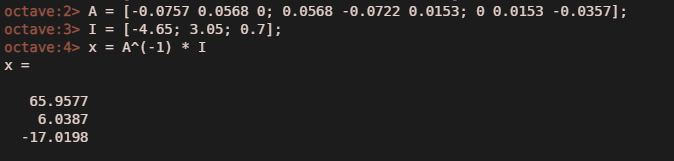
\includegraphics[scale=0.5]{picturesFor3Uloha/2.png}
    \begin{quote}
        \centering
        $\phi A = 65.9577 \Vo$ \\ 
        $\phi B = 6.0387 \Vo$ \\
        $\phi C = -17.0198 \Vo$ \\ 
        \medskip
        \medskip
         $I_{R3} = \dfrac{(\phi B - \phi C)}{R_3} = \dfrac{( 6.0387\Vo + 17.0198 \Vo)}{65\Omega} = 0.3547\Am$ \\~\\
         $U_{R3} = I_{R3} * R_3 = 0.3547\Am * 65\Omega = 23.0587\Vo$
    \end{quote}
\end{figure}